\documentclass[aspectratio=169]{beamer}
\setbeamertemplate{navigation symbols}{}
\usepackage{color,amsmath,comment, subfigure}
\usepackage{booktabs}
\usepackage{url}

%\setbeameroption{show notes}

%%%%%%%%%%%%%%%%%%%%%%%%%%
\title[]{Class 7: Social search}
\author[]{Matthew J. Salganik}
\institute[]{Sociology 204: Social Networks, Spring 2021\\Princeton University}
\date[]{
1/2: Search in the small world problem
\vfill

\begin{flushleft}
\vspace{0.6in}

\includegraphics[width=0.1\textwidth]{figures/cc.png}
\end{flushleft}

}

% TODO: SWBAT
% TODO: Work on part about ultra-metric distance

\begin{document}
%%%%%%%%%%%%%%%%%%%%%%%%%%%
\frame{\titlepage}
%%%%%%%%%%%%%%%%%%%%%%%%%%%
\begin{comment}
\begin{frame}

SWBAT:
\begin{enumerate}
\end{enumerate}

\end{frame}
\end{comment}
%%%%%%%%%%%%%%%%%%%%%%%%
\begin{frame}
\frametitle{Review}

\begin{itemize}
\item sometimes the edges that don't exist are as important as the edges that do exist
\pause
\item affiliation networks (people and groups) help us understand patterns in personal network structure
\pause
\item compare and contrast psychological vs sociological explanations for network structure 
\pause
\item sociological principles can shape the design of technical systems
\end{itemize}

\note{
Foci help us understand search
}

\end{frame}
%%%%%%%%%%%%%%%%%%%%%%%%%%%
\begin{frame}

Travers and Milgram showed two things
\begin{enumerate}
\item short paths exist
\item people can find them using only local information
\end{enumerate}

\pause 

Watts distinguishes between
\begin{itemize}
\item Broadcast search (what the six degrees website did in your wikipedia assignment)
\item Directed search (what you did in your wikipedia assignment)
\end{itemize}

\pause 
\vfill
How is it that directed search ever works?

\note{
This class we are going to learn about some models about what makes networks searchable and we are going to read about a real search problem.

Search for an abortionist is in-between broadcast and directed

Beta model only shows that short paths exist not that we can find them

Why should we expect directed search to be hard.  We know about our friends and maybe some beyond that, but our information is very local.
}


\end{frame}
%%%%%%%%%%%%%%%%%%%%%%%
\begin{frame}

\begin{figure}
  \centering
  \includegraphics[width=0.8\textwidth]{figures_book/3_6}
\end{figure}

\note{
Kleinberg figured out that directed search (not broadcast search) was impossible in Watts/Strogatz model because shortcuts are random (not related to underlying geometry).  So Kleinberg made a new model.  Not surprising that as a CS prof he was interested in search, at about the same time as google he had the idea of using links (instead of page content) to rank search, but he simply published his idea and moved on
}

\end{frame}
%%%%%%%%%%%%%%%%%%%%%%%
\begin{frame}

\begin{figure}
  \centering
  \includegraphics[width=0.8\textwidth]{figures_book/5_1}
\end{figure}

\end{frame}
%%%%%%%%%%%%%%%%%%%%%%%
\begin{frame}


\setcounter{subfigure}{0}
\begin{figure}
  \centering
     \subfigure[]{
     \includegraphics[width=0.45\textwidth]{figures_book/5_2}}
  \hspace{0in}
    \subfigure[]{
    \includegraphics[width=0.45\textwidth]{figures_book/5_3}}
\end{figure}

\begin{itemize}
\item low $\gamma$: lots of long connections, but networks not searchable
\pause
\item  $\gamma = 2$: same number of ties at all length scales, networks searchable 
\pause
\item high $\gamma$: no long connections, no short paths
\end{itemize}

\note{
x-axis: log distance
y-axis: probably of link that long

When gamma is too big graph is unsearchable, when gamma is too small not enough big shortcuts.  

Notice how this model again involves trade-off between order and randomness (similar to beta model)

Weird that the model only works for one value.  Think about parameterization
}

\end{frame}
%%%%%%%%%%%%%%%%%%%%%%%
\begin{frame}

\begin{figure}
  \centering
  
\includegraphics[width=0.8\textwidth]{figures/kleinberg_navigation_2000_title}
\end{figure}

\vfill

\url{http://dx.doi.org/10.1038/35022643}

\note{
full details
}

\end{frame}
%%%%%%%%%%%%%%%%%%%%%%%
\begin{frame}

\begin{figure}
  \centering
  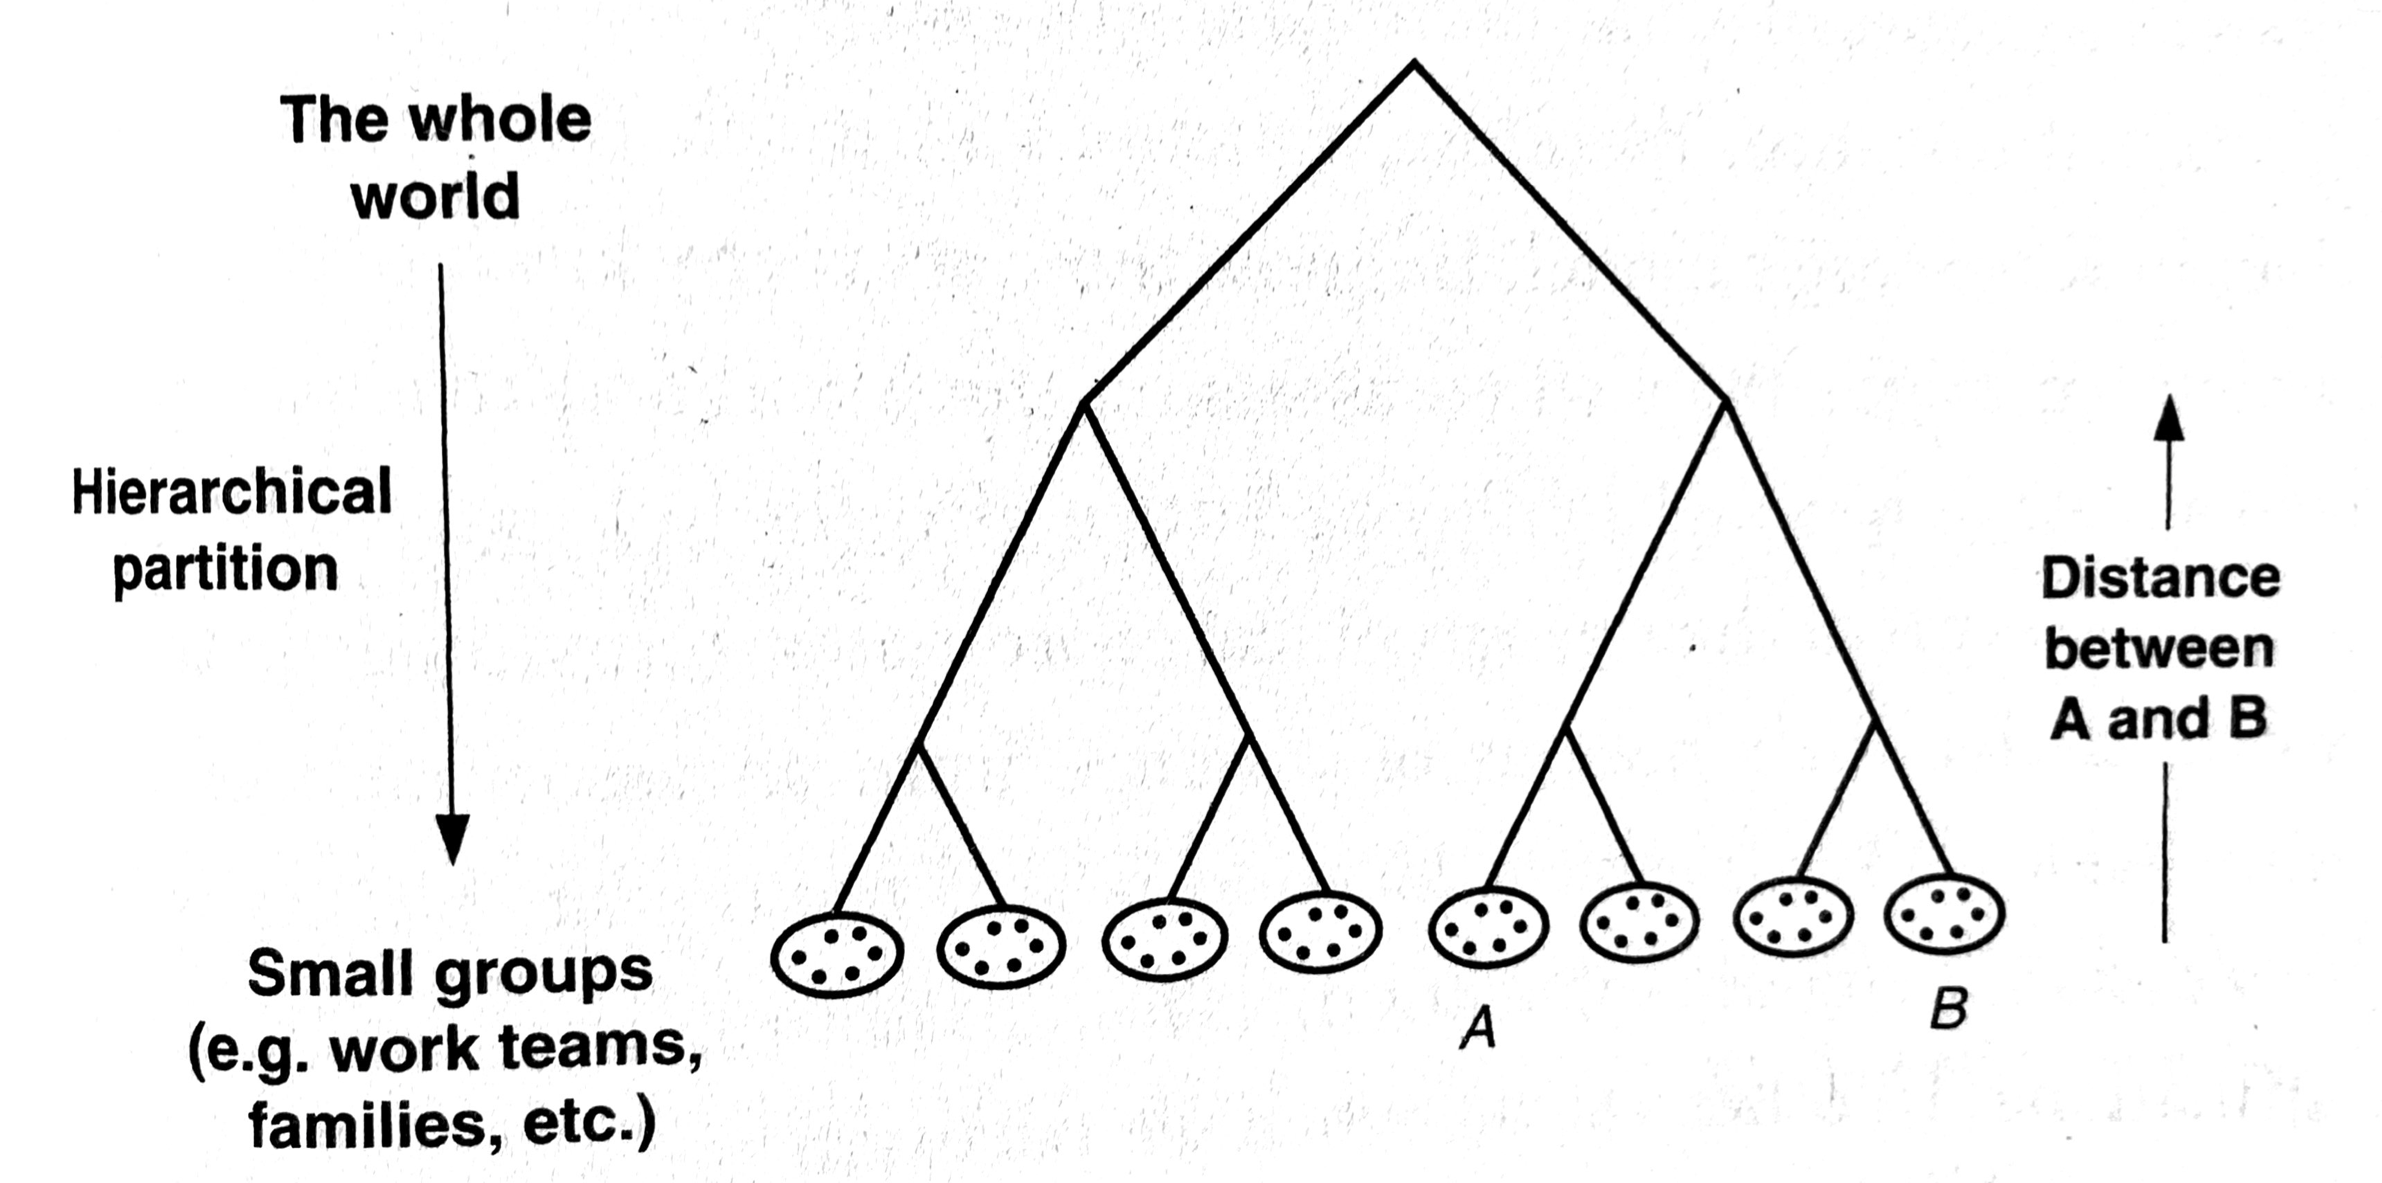
\includegraphics[width=0.9\textwidth]{figures/5_6}
\end{figure}

\note{
Nested groups, dorms nested within residential colleges
}

\end{frame}
%%%%%%%%%%%%%%%%%%%%%%%
\begin{frame}

\begin{figure}
  \centering
  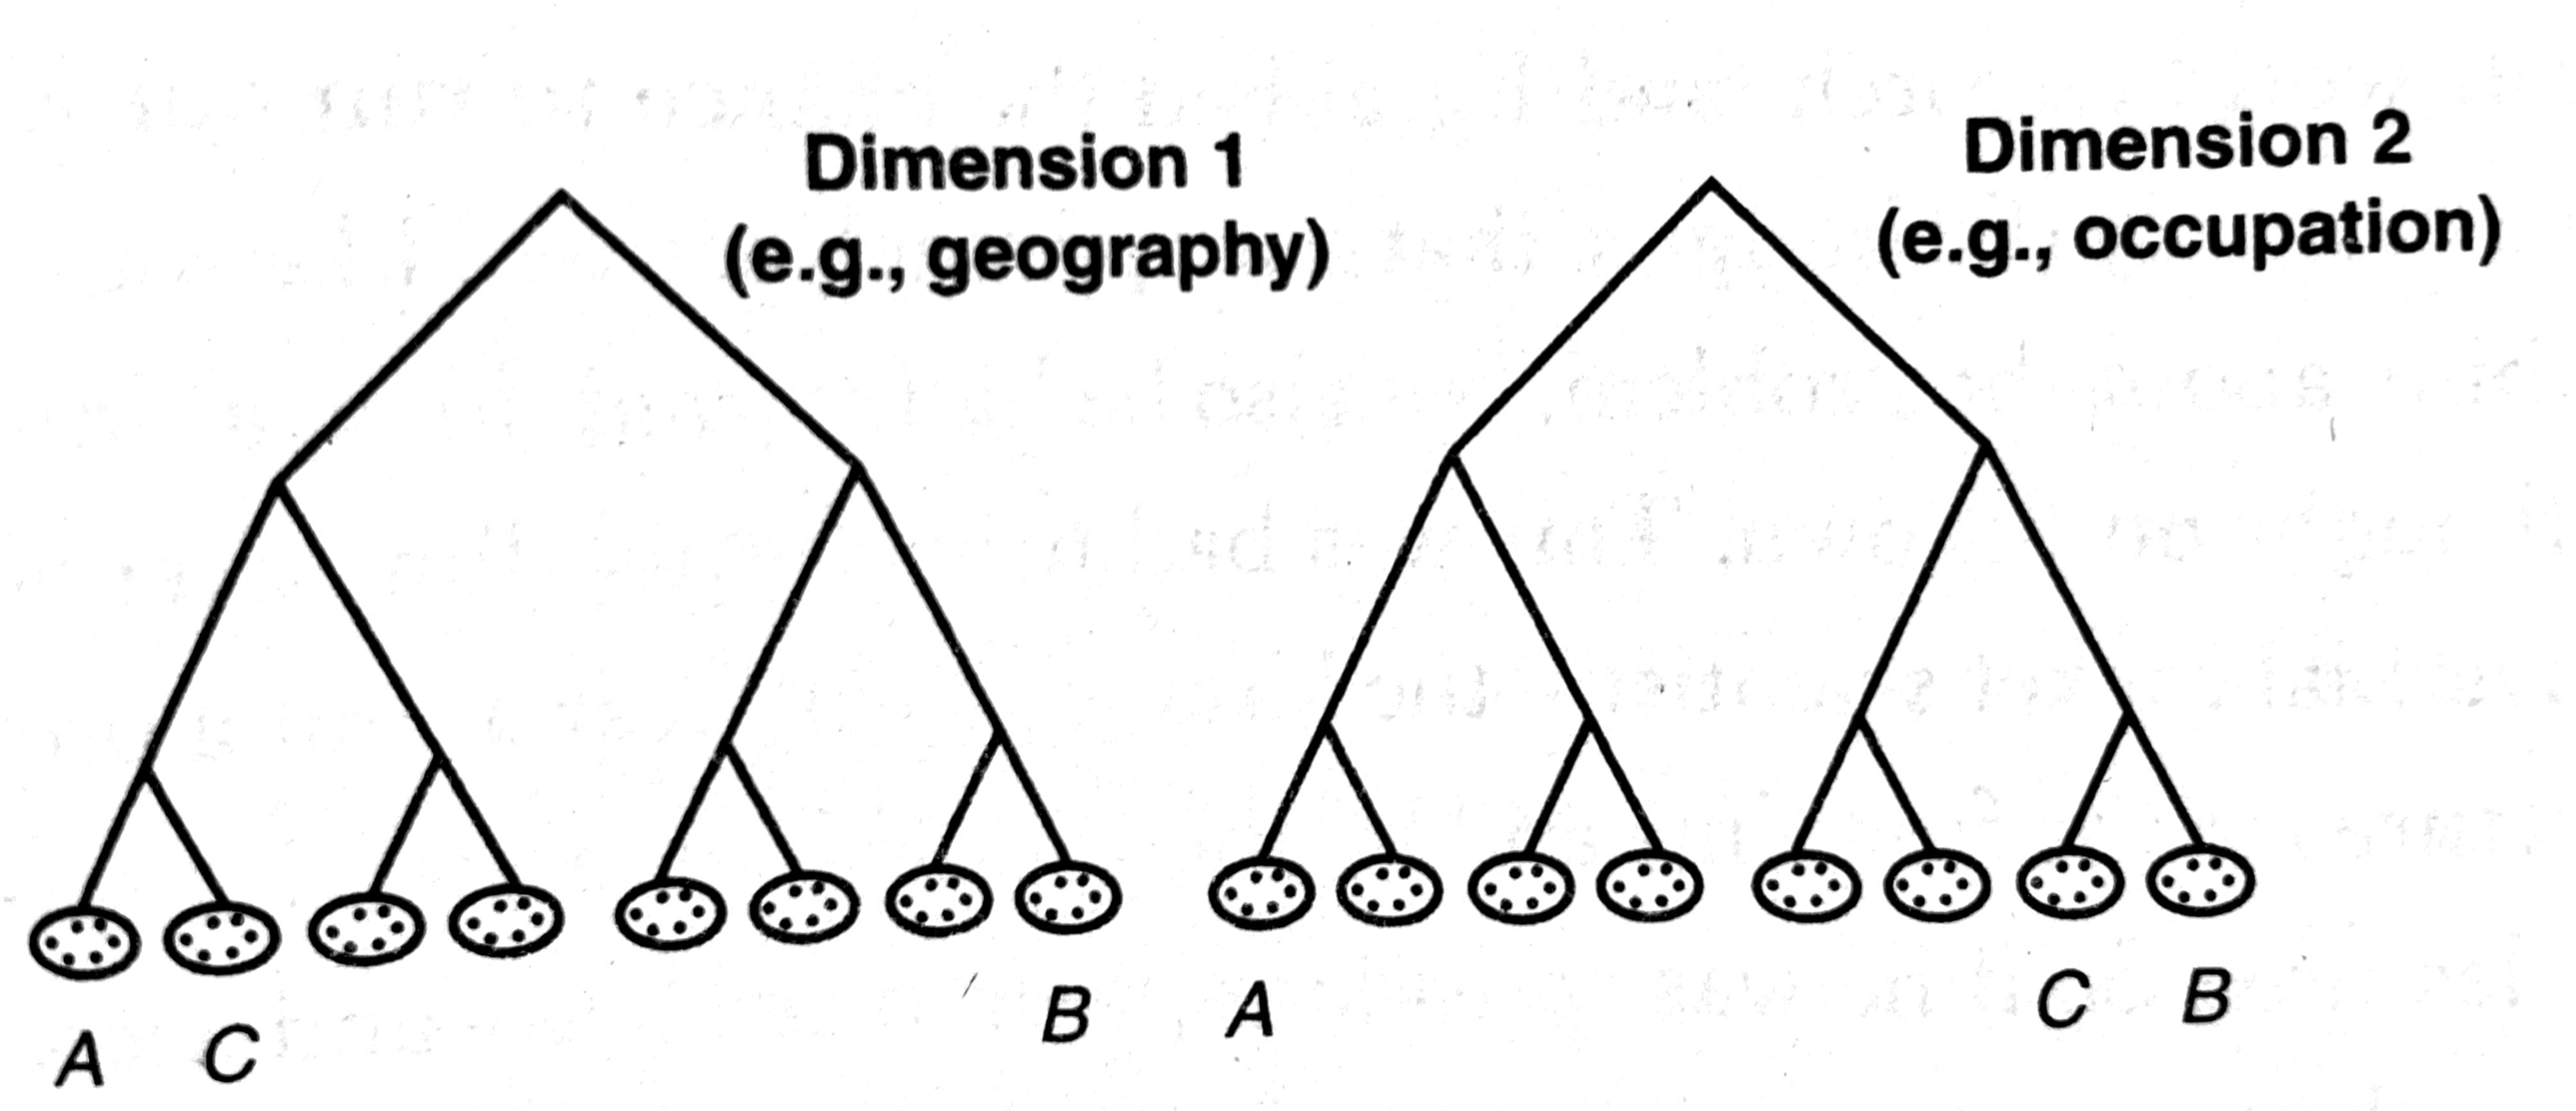
\includegraphics[width=0.9\textwidth]{figures/5_7}
\end{figure}

\note{
Richer notion of distance is required along multiple dimensions.  For example, you may seem far from Duncan.  You live in a different place and you have a different occupation.  But, you are close to me (we live in the same place) and I am close to Duncan (we have the same occupation).   So, you might feel far from Duncan socially, but not in a network sense.
}

\end{frame}
%%%%%%%%%%%%%%%%%%%%%%%
\begin{frame}

\begin{figure}
  \centering
  \includegraphics[width=0.8\textwidth]{figures/5_8}
\end{figure}

We will not define axes. Details of this model are not as important as the other models we have learned about.

\note{networks are searchable for a wide range of values

Also, involves mix of structure and randomness
}

\end{frame}
%%%%%%%%%%%%%%%%%%%%%%%%%%
\begin{frame}

\begin{figure}
  \centering
  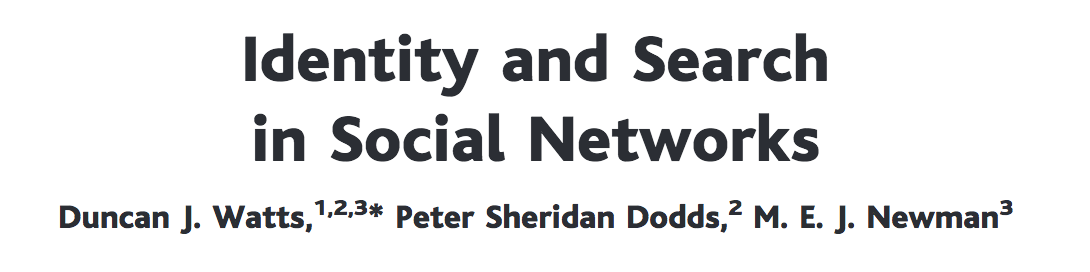
\includegraphics[width=0.8\textwidth]{figures/watts_identity_2002_title}
\end{figure}

\vfill

\url{http://dx.doi.org/10.1126/science.1070120}

\note{networks are searchable for a wide range of values}

\end{frame}
%%%%%%%%%%%%%%%%%%%%%%%%%%
\begin{frame}

\begin{figure}
  \centering
  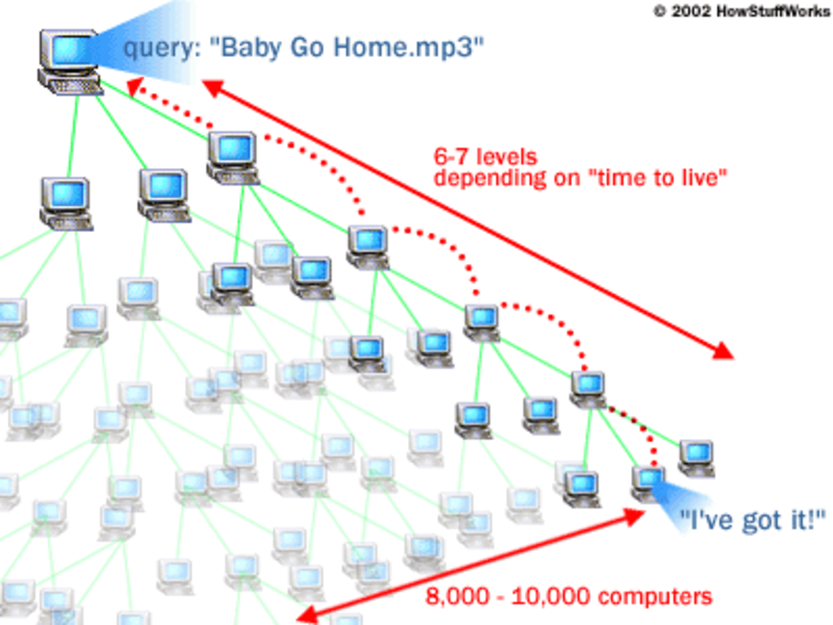
\includegraphics[width=0.6\textwidth]{figures/how_gnutella_works}
\end{figure}

\tiny{\url{http://computer.howstuffworks.com/file-sharing3.htm}}

\note{
Here's how peer-to-peer networks work, this involves search.

You can do broadcast search to like for My Heart Will Go On (titanic)
}

\end{frame}
%%%%%%%%%%%%%%%%%%%%%%%%%%%
\begin{frame}

Who cares about social search?

\end{frame}

\end{document}
